  \tcbset{
    subfigframe/.style={
        enhanced, sharp corners, boxrule=0.5pt,
        colback=white, colframe=black, coltitle=black,
        left=0pt, right=0pt, top=5pt, bottom=0pt,
        fonttitle=\bfseries,
        attach boxed title to top left={xshift=6pt, yshift=-\tcboxedtitleheight/2},
        boxed title style={
            sharp corners, boxrule=0.5pt,
            colback=white, colframe=black,
            size=small,
        },
    }
}

\begin{figure*}
    \begin{subfigure}{\textwidth}
        \begin{tcolorbox}[subfigframe, title= (A) WSI preprocessing]
            \centering
            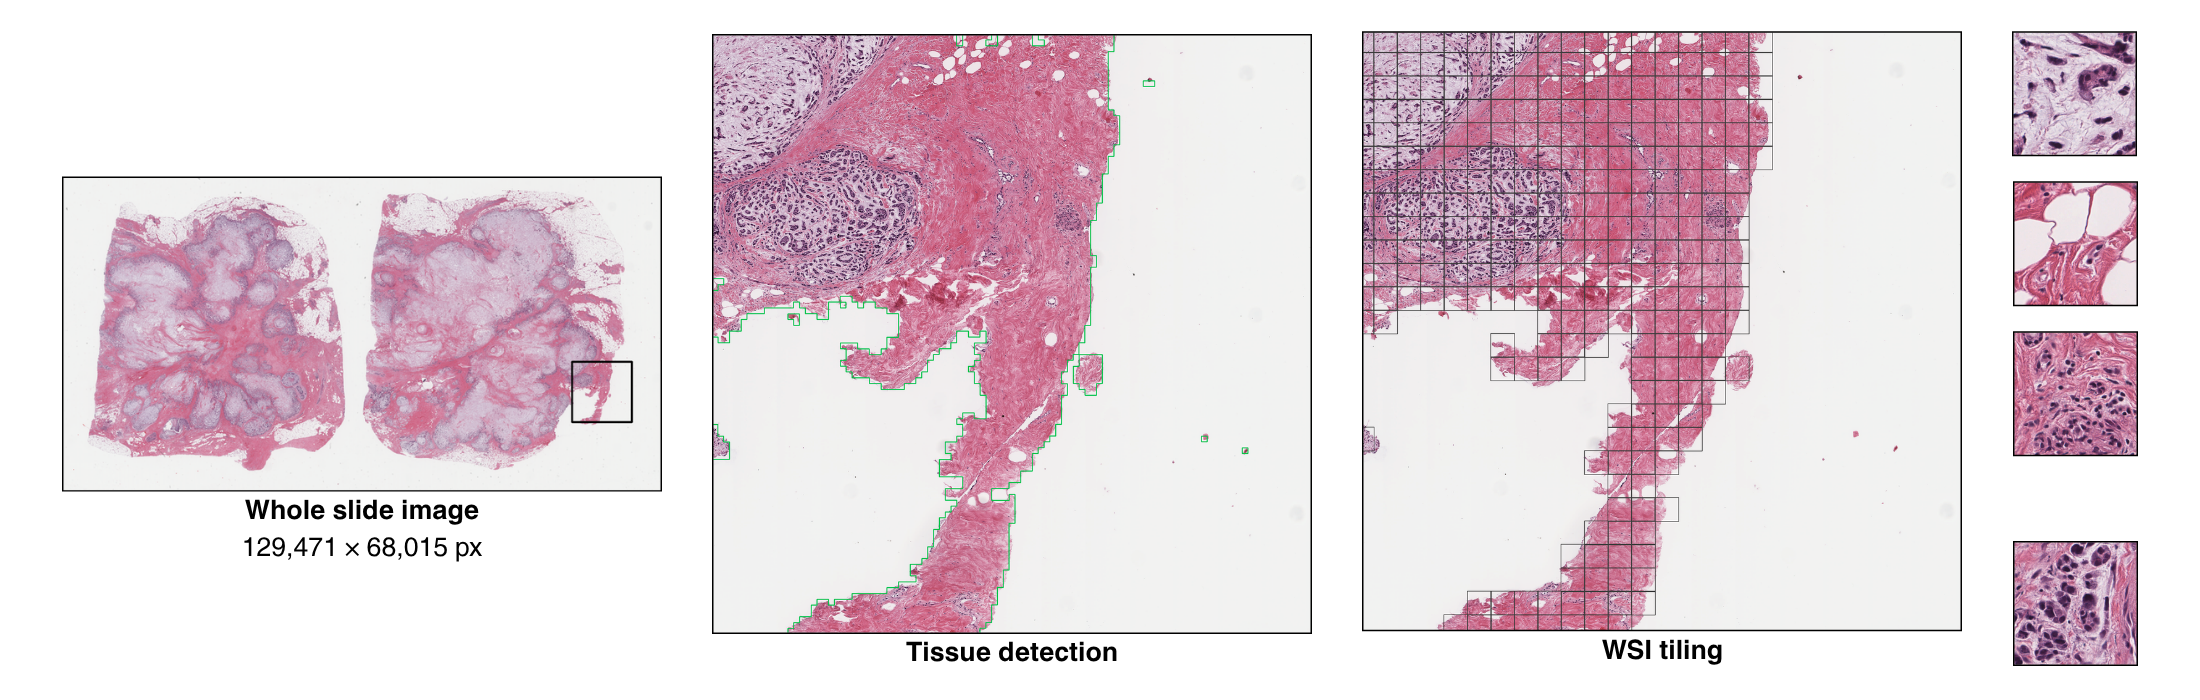
\includegraphics[width=1.0\linewidth]{images/tissue_tiling.png}
        \end{tcolorbox}
    \end{subfigure}
    \par\vspace{0.5em}\par
    \begin{subfigure}{\textwidth}
        \begin{tcolorbox}[subfigframe, title= (B) Tile-level feature extraction]
            \centering
            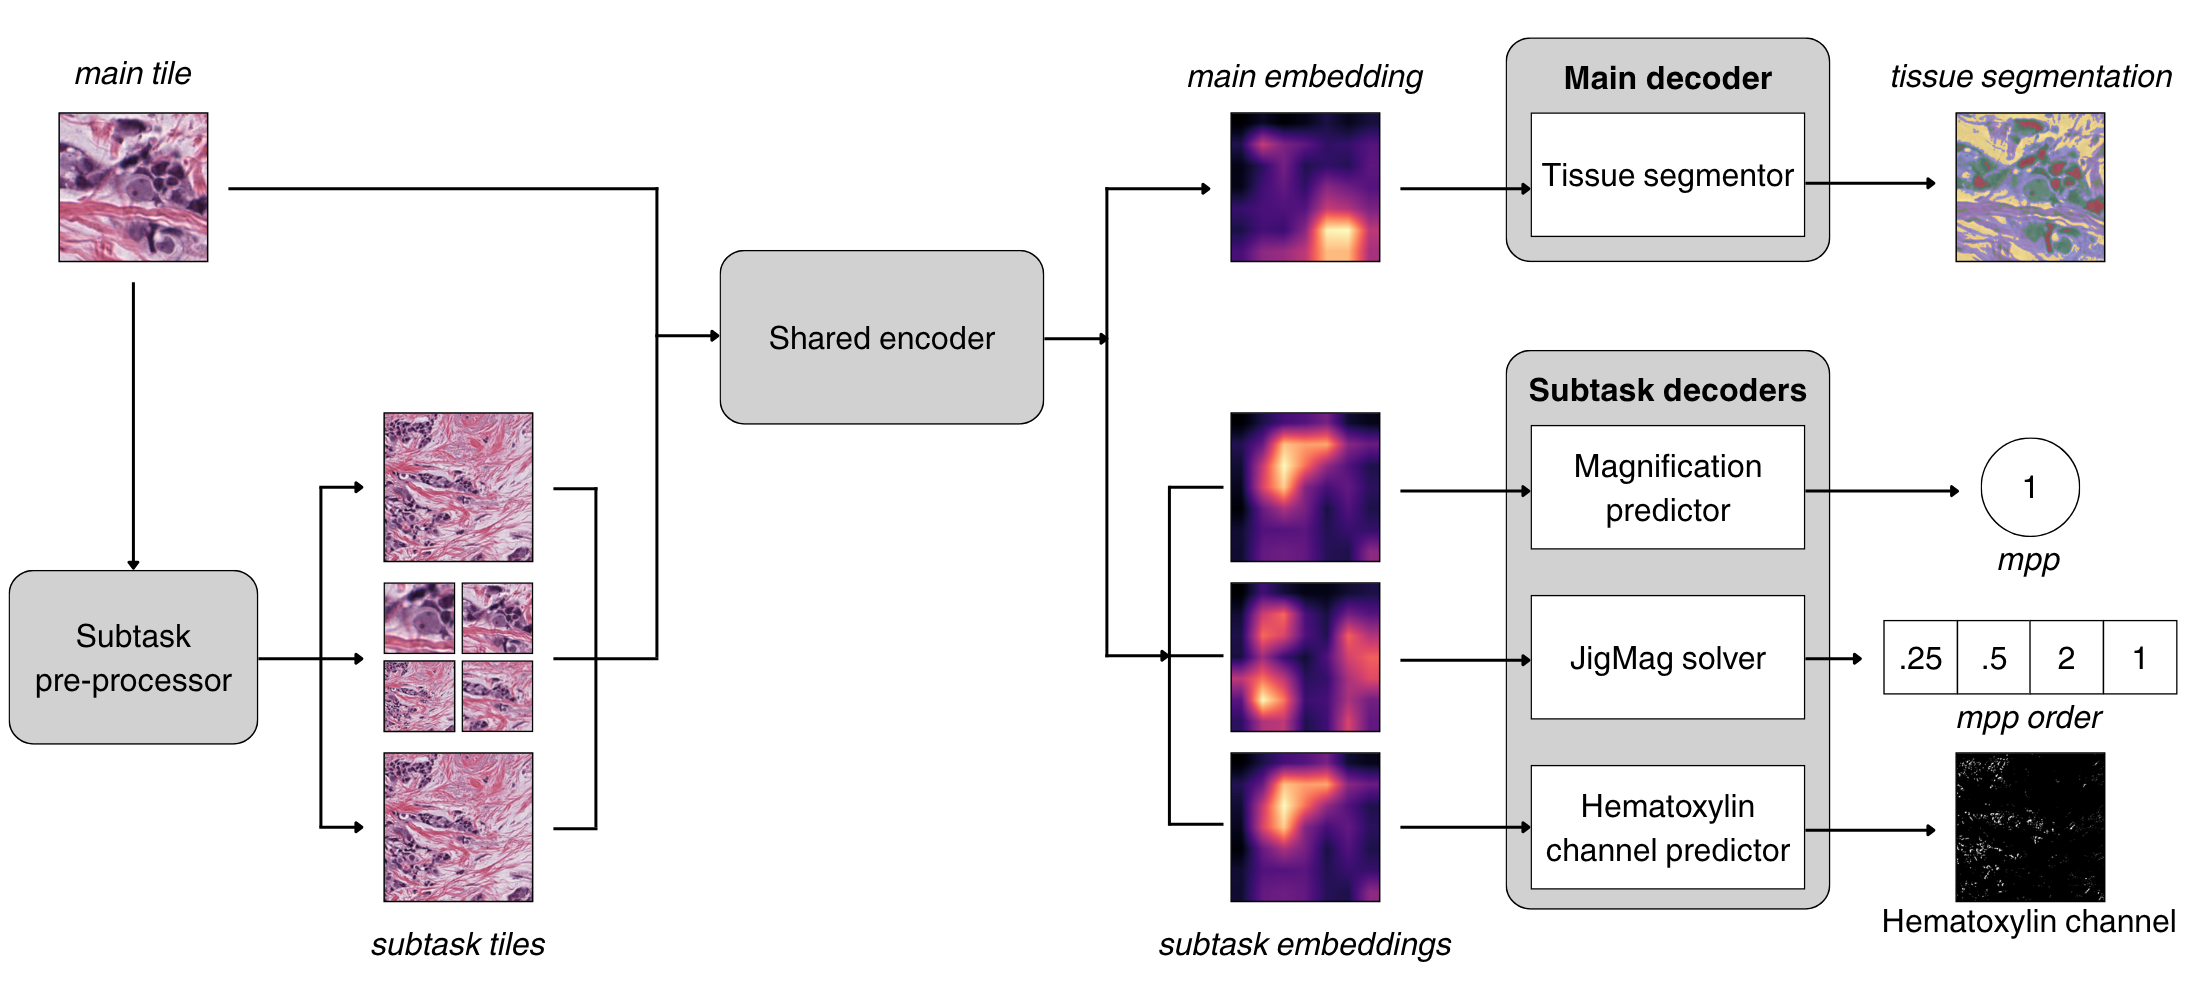
\includegraphics[width=1.0\linewidth]{images/tile_level_feature_extraction.png}
        \end{tcolorbox}
    \end{subfigure}
    \caption{}\label{fig:method-overview}
\end{figure*}

\begin{figure*}
    \centering
    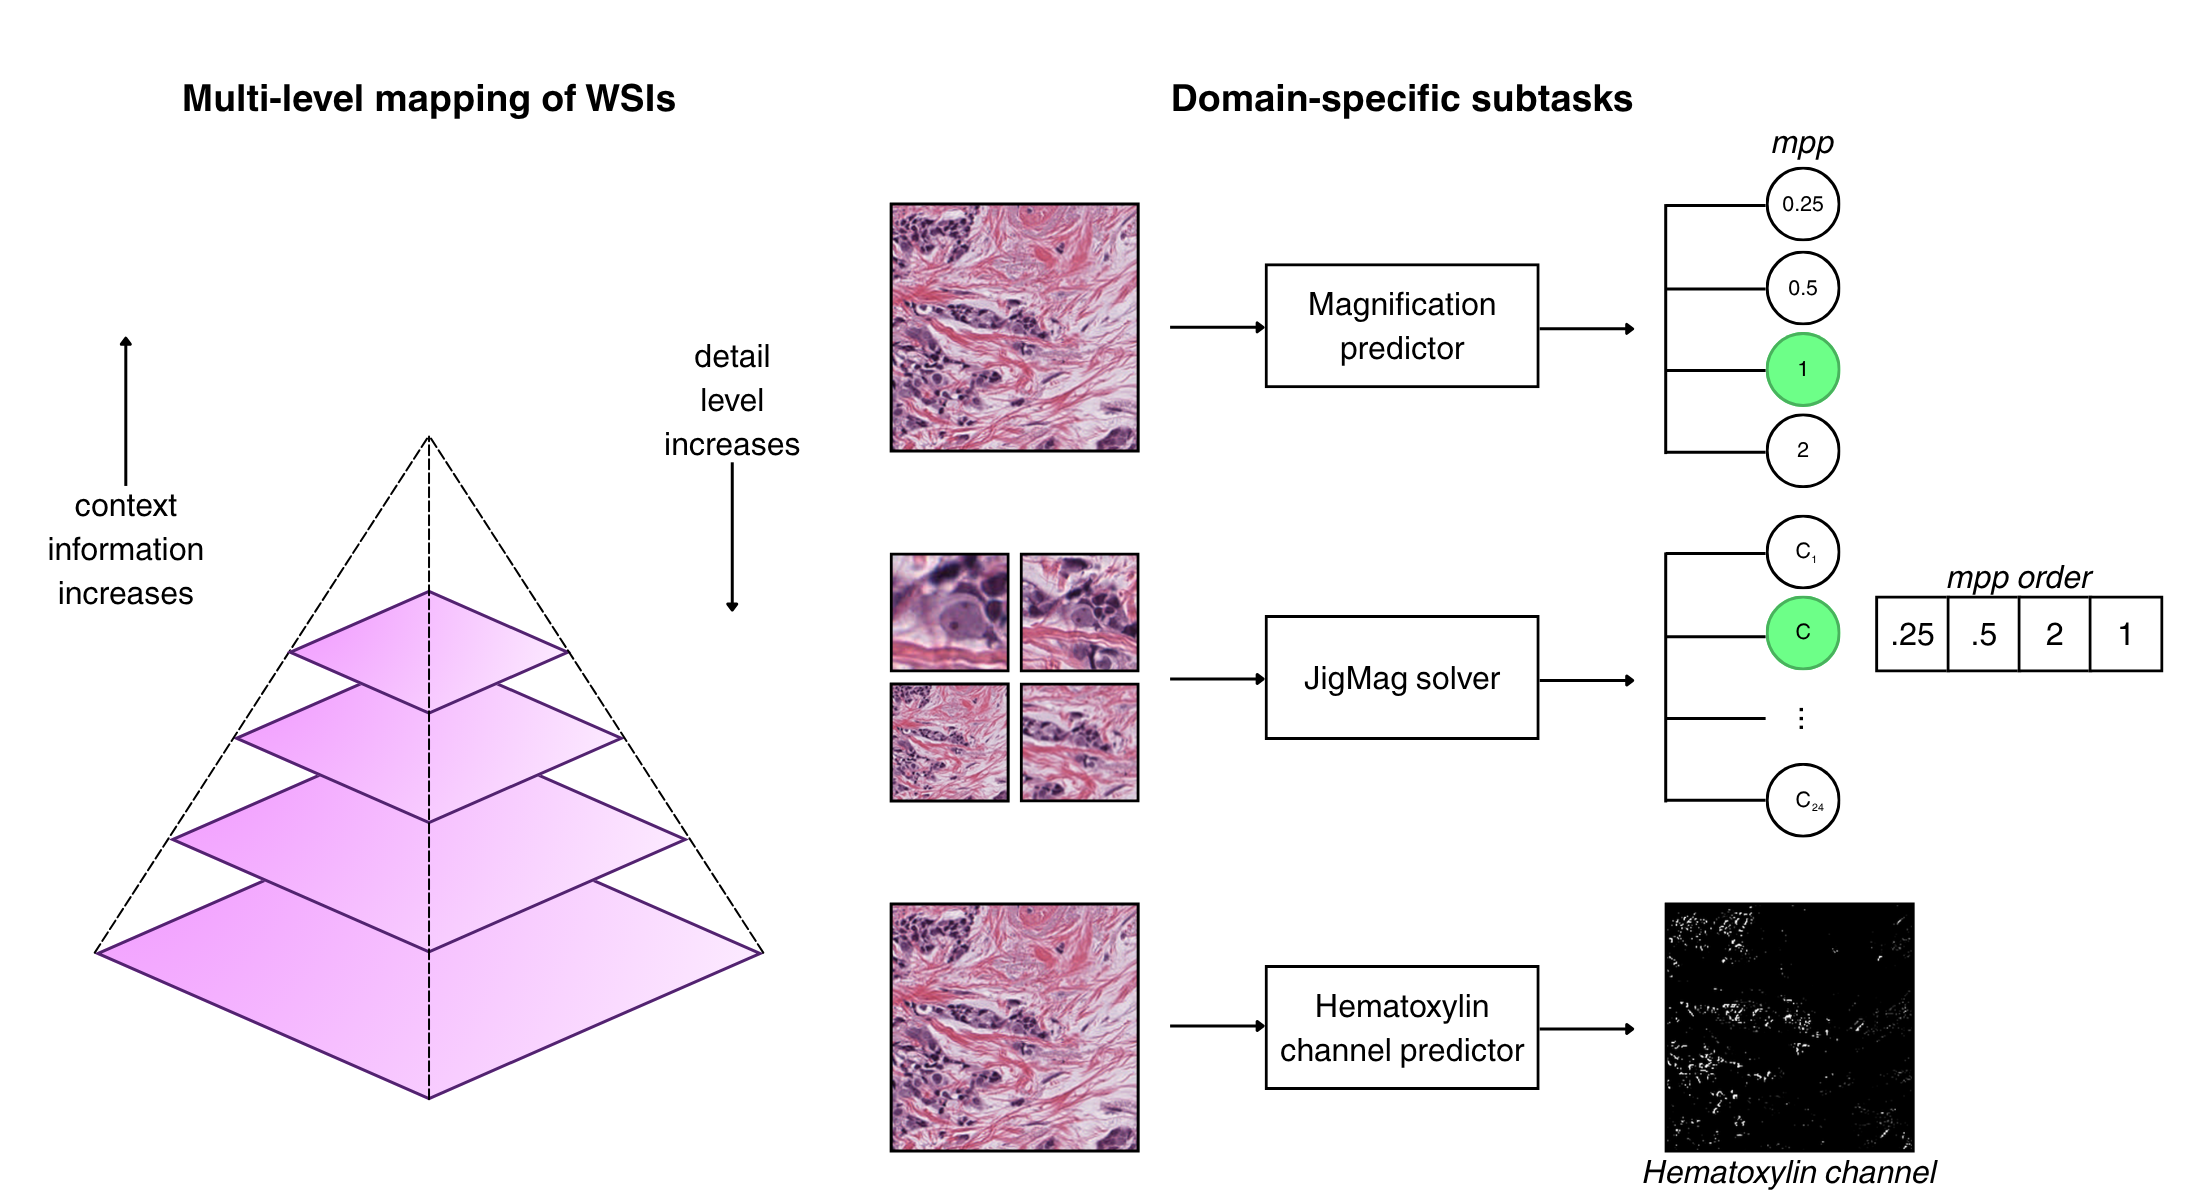
\includegraphics[width=1.0\linewidth]{images/tile_level_pretext_tasks.png}
    \caption{}\label{fig:tile-subtasks}
\end{figure*}